\documentclass[a4paper,12pt]{article}
\usepackage[utf8]{inputenc}
\usepackage{geometry}
\usepackage{booktabs}
\usepackage{graphicx}
\usepackage{float}
\usepackage{enumitem}
\geometry{left=2.5cm, right=2.5cm, top=2.5cm, bottom=2.5cm}

\title{\textbf{Task 2: MIP Data Analysis}}
\author{Computer Data Analysis Course}
\date{\today}

\begin{document}

\maketitle

\section*{Step 1: Dataset Selection}

I selected the \textbf{MIP 2016} wave from the Mannheim Innovation Panel (2009--2016). The dataset contains 2,000 German firms with 96 variables covering innovation activities, digitalization, and firm characteristics.

\section*{Step 2: Descriptive Statistics}

Table \ref{tab:desc} shows descriptive statistics for all variables used in the analysis (regression sample, N = 1,023).

\begin{table}[H]
\centering
\caption{Descriptive Statistics (N = 1,023)}
\label{tab:desc}
\begin{tabular}{lrrrr}
\toprule
Variable & Mean & Std. Dev. & Min & Max \\
\midrule
\textit{Outcome} & & & & \\
novor & 0.121 & 0.327 & 0 & 1 \\
\addlinespace
\textit{Main Explanatory (Index)} & & & & \\
digitalization (index) & 0.884 & 0.665 & 0 & 3 \\
\addlinespace
\textit{Controls} & & & & \\
ost (East Germany) & 0.346 & 0.476 & 0 & 1 \\
bges (employees) & 252.1 & 421.5 & 1 & 3500 \\
lp (labor productivity) & 0.260 & 0.175 & 0.006 & 0.600 \\
ex (total exports) & 3.793 & 17.701 & 0 & 315.07 \\
qual (quality improvement) & 0.138 & 0.345 & 0 & 1 \\
\bottomrule
\end{tabular}
\end{table}

About 12.1\% of firms introduced novel innovations. The digitalization index (average of 11 digital technology usage variables) has a mean of 0.88 on a 0-3 scale. For control variables: 34.6\% of firms are in East Germany, average firm size is 252 employees, average labor productivity is 0.26, average exports are 3.79 (highly skewed: 59.7\% have zero exports, mean = 9.42 for exporters), and 13.8\% of firms achieved quality improvements through process innovations.

\section*{Step 3: Key Variables}

\textbf{Outcome variable:}
\begin{itemize}
    \item \textbf{Novel product innovation -- innovation without forerunner products (2013--2015)} -- binary variable indicating whether the firm introduced a product innovation that had no predecessor product (i.e., a radically new innovation, not just an improvement of existing products). (No novel innovation = 0, Novel innovation introduced = 1).
    \item \textbf{Name in dataset:} \texttt{novor}
    \item \textbf{Why chosen:} This variable captures \textit{radical} innovations rather than incremental improvements. It is a stricter measure than general product innovation (\texttt{pd}) because it excludes innovations that were merely improvements of existing products. The binary nature (0/1) makes it suitable for logit model.
\end{itemize}

\textbf{Main explanatory variable:}
\begin{itemize}
    \item \textbf{Digitalization index} -- Composite measure created from 11 digital technology usage variables (average of digia1--digia11):
    \begin{itemize}
        \item digia1: Digital interconnection within production
        \item digia2: Digital interconnection between production units
        \item digia3: Digital interconnection with customers
        \item digia4: Digital interconnection with suppliers
        \item digia5: Teleworking
        \item digia6: Software-based communication
        \item digia7: Intranet-based platforms
        \item digia8: E-commerce
        \item digia9: Social media
        \item digia10: Cloud computing
        \item digia11: Big data analysis
    \end{itemize}
    \item \textbf{Name in dataset:} \texttt{digia1}--\texttt{digia11} (combined into index)
    \item \textbf{Why chosen:} These variables directly measure current usage of digital technologies in the firm. Creating an index captures the overall intensity of digitalization across multiple dimensions.
\end{itemize}

\textbf{Control variables:}
\begin{itemize}
    \item \textbf{Firm size} -- Number of full-time employees. Part-time employees and apprentices are counted as 0.5 of a full-time post. \textbf{Name in dataset:} \texttt{bges}
    
    \item \textbf{East/West Germany location} -- Regional location of the firm. (Western Germany = 0, Eastern Germany = 1). \textbf{Name in dataset:} \texttt{ost}
    
    \item \textbf{Total exports (2016)} -- Total amount exported in 2016 (standardized units). This is a continuous variable where 59.7\% of firms have zero exports and 40.3\% have positive exports (mean = 9.42 for exporters, max = 315.07). \textbf{Name in dataset:} \texttt{ex}
    
    \item \textbf{Labor productivity} -- Labor productivity measured as output per worker (range: 0.006 to 0.600). \textbf{Name in dataset:} \texttt{lp}
    
    \item \textbf{Quality improvement by process innovations} -- Indicator for whether the firm achieved quality improvements through process innovations. (No = 0, Yes = 1). \textbf{Name in dataset:} \texttt{qual}
    
    \item \textbf{Industry dummies} -- 21 economic sector (WZ) classification dummies to control for industry-specific effects. \textbf{Name in dataset:} \texttt{branche}
\end{itemize}

\textbf{Why logit model:} The outcome variable \texttt{novor} is binary (0 or 1 only), making logistic regression appropriate instead of OLS linear regression.

\textbf{Expected relationship between these variables:}
\begin{itemize}
    \item Firms with higher digitalization (more intensive use of digital technologies) are expected to have a higher probability of introducing novel product innovations compared to firms with low digitalization.
    \item The relationship is expected to be positive: as digitalization increases, innovation probability should increase.
\end{itemize}

\textbf{Theoretical mechanisms underlying this relationship:}
\begin{itemize}
    \item \textbf{Knowledge management:} Firms that use digital software intensively can better store, organize, and share knowledge within the organization. This makes it easier to combine existing knowledge in new ways and develop innovative products. Firms with low digitalization struggle with knowledge silos and information fragmentation.
    
    \item \textbf{Process efficiency:} Digital tools streamline R\&D processes, reduce administrative burden, and accelerate product development cycles. Firms with high software usage can move from idea to market faster, increasing their innovation output.
    
    \item \textbf{Market intelligence:} Digital platforms provide better access to customer feedback, market trends, and competitor information. Firms using these tools can identify innovation opportunities more effectively and develop products that better match market needs.
    
    \item \textbf{Collaboration:} Software tools enable better internal and external collaboration. R\&D teams can work more effectively together, and firms can collaborate with external partners (universities, suppliers, customers) on innovation projects.
\end{itemize}

\section*{Step 4: Regression Analysis}

Table \ref{tab:reg} presents four logistic regression models with increasing controls.

\begin{table}[H]
\centering
\caption{Logistic Regression Results: Novel Product Innovation}
\label{tab:reg}
\begin{tabular}{lcccc}
\toprule
 & (1) & (2) & (3) & (4) \\
 & Baseline & + Controls & + Qual/Ex & + Industry FE \\
\midrule
digitalization & 0.137*** & 0.116*** & 0.038** & 0.034*** \\
 & (0.015) & (0.015) & (0.012) & (0.013) \\
ost & & 0.039 & 0.046** & 0.052** \\
 & & (0.020) & (0.016) & (0.016) \\
bges & & 0.001*** & 0.000*** & 0.000*** \\
 & & (0.000) & (0.000) & (0.000) \\
lp & & 0.018 & 0.002 & 0.016 \\
 & & (0.056) & (0.046) & (0.051) \\
ex & & & 0.000 & 0.000 \\
 & & & (0.001) & (0.001) \\
qual & & & 0.570*** & 0.557*** \\
 & & & (0.024) & (0.025) \\
Industry FE & No & No & No & Yes (21) \\
Observations & 1023 & 1023 & 1023 & 1023 \\
Pseudo R² & 0.077 & 0.129 & 0.448 & 0.470 \\
\bottomrule
\end{tabular}
\par
\small Notes: Logit coefficients with standard errors in parentheses. *** p$<$0.01, ** p$<$0.05, * p$<$0.10. Industry fixed effects (21 industries) included in column (4).
\end{table}

\textbf{Result:} Digitalization has a positive and statistically significant effect on novel innovation probability (coef = 0.034, p = 0.007). The hypothesis IS supported -- firms with higher digitalization are more likely to introduce novel innovations.

\section*{Step 5: Inference with Robust Standard Errors}

\begin{table}[H]
\centering
\caption{Comparison: Non-Robust vs. Robust Standard Errors}
\begin{tabular}{lrrrr}
\toprule
Variable & \multicolumn{2}{c}{Std. Error} & \multicolumn{2}{c}{P-value} \\
\cmidrule(lr){2-3} \cmidrule(lr){4-5}
 & Non-robust & Robust (HC1) & Non-robust & Robust \\
\midrule
digitalization & 0.0126 & 0.0128 & 0.007 & 0.008 \\
ost & 0.0163 & 0.0160 & 0.001 & 0.001 \\
bges & 0.000075 & 0.000103 & 0.0003 & 0.0085 \\
qual & 0.0248 & 0.0444 & $<$0.001 & $<$0.001 \\
\bottomrule
\end{tabular}
\end{table}

\textbf{Comparison:}
\begin{itemize}
    \item Robust standard errors are slightly larger for some variables (bges increases by about 37\%)
    \item P-values remain essentially unchanged for digitalization (0.007 $\rightarrow$ 0.008)
    \item Digitalization remains statistically significant (p = 0.008 with robust SE)
    \item Qualification and East Germany location remain statistically significant
\end{itemize}

\textbf{Conclusion:} Main findings are robust to heteroskedasticity-robust inference.

\section*{Step 6: Interaction Effects}

I added an interaction term: \texttt{digitalization} $\times$ \texttt{bges} (digitalization $\times$ firm size).

\textbf{Why moderation is expected:}
\begin{itemize}
    \item Larger firms typically have more complementary resources (R\&D budgets, specialized personnel, dedicated innovation teams) that could enable them to better leverage digital technologies for innovation.
    
    \item Small firms may adopt digital technologies but lack the organizational capacity to translate digital tools into innovation outcomes.
    
    \item Larger firms may have better processes and infrastructure to implement digital technologies effectively, leading to stronger innovation returns from the same level of digitalization.
\end{itemize}

\textbf{Result:} The interaction term is NOT statistically significant (coef = $-$0.000137, p = 0.23). The effect of digitalization on innovation does NOT vary by firm size in this sample.

\section*{Step 7: Visualization}

\begin{figure}[H]
\centering
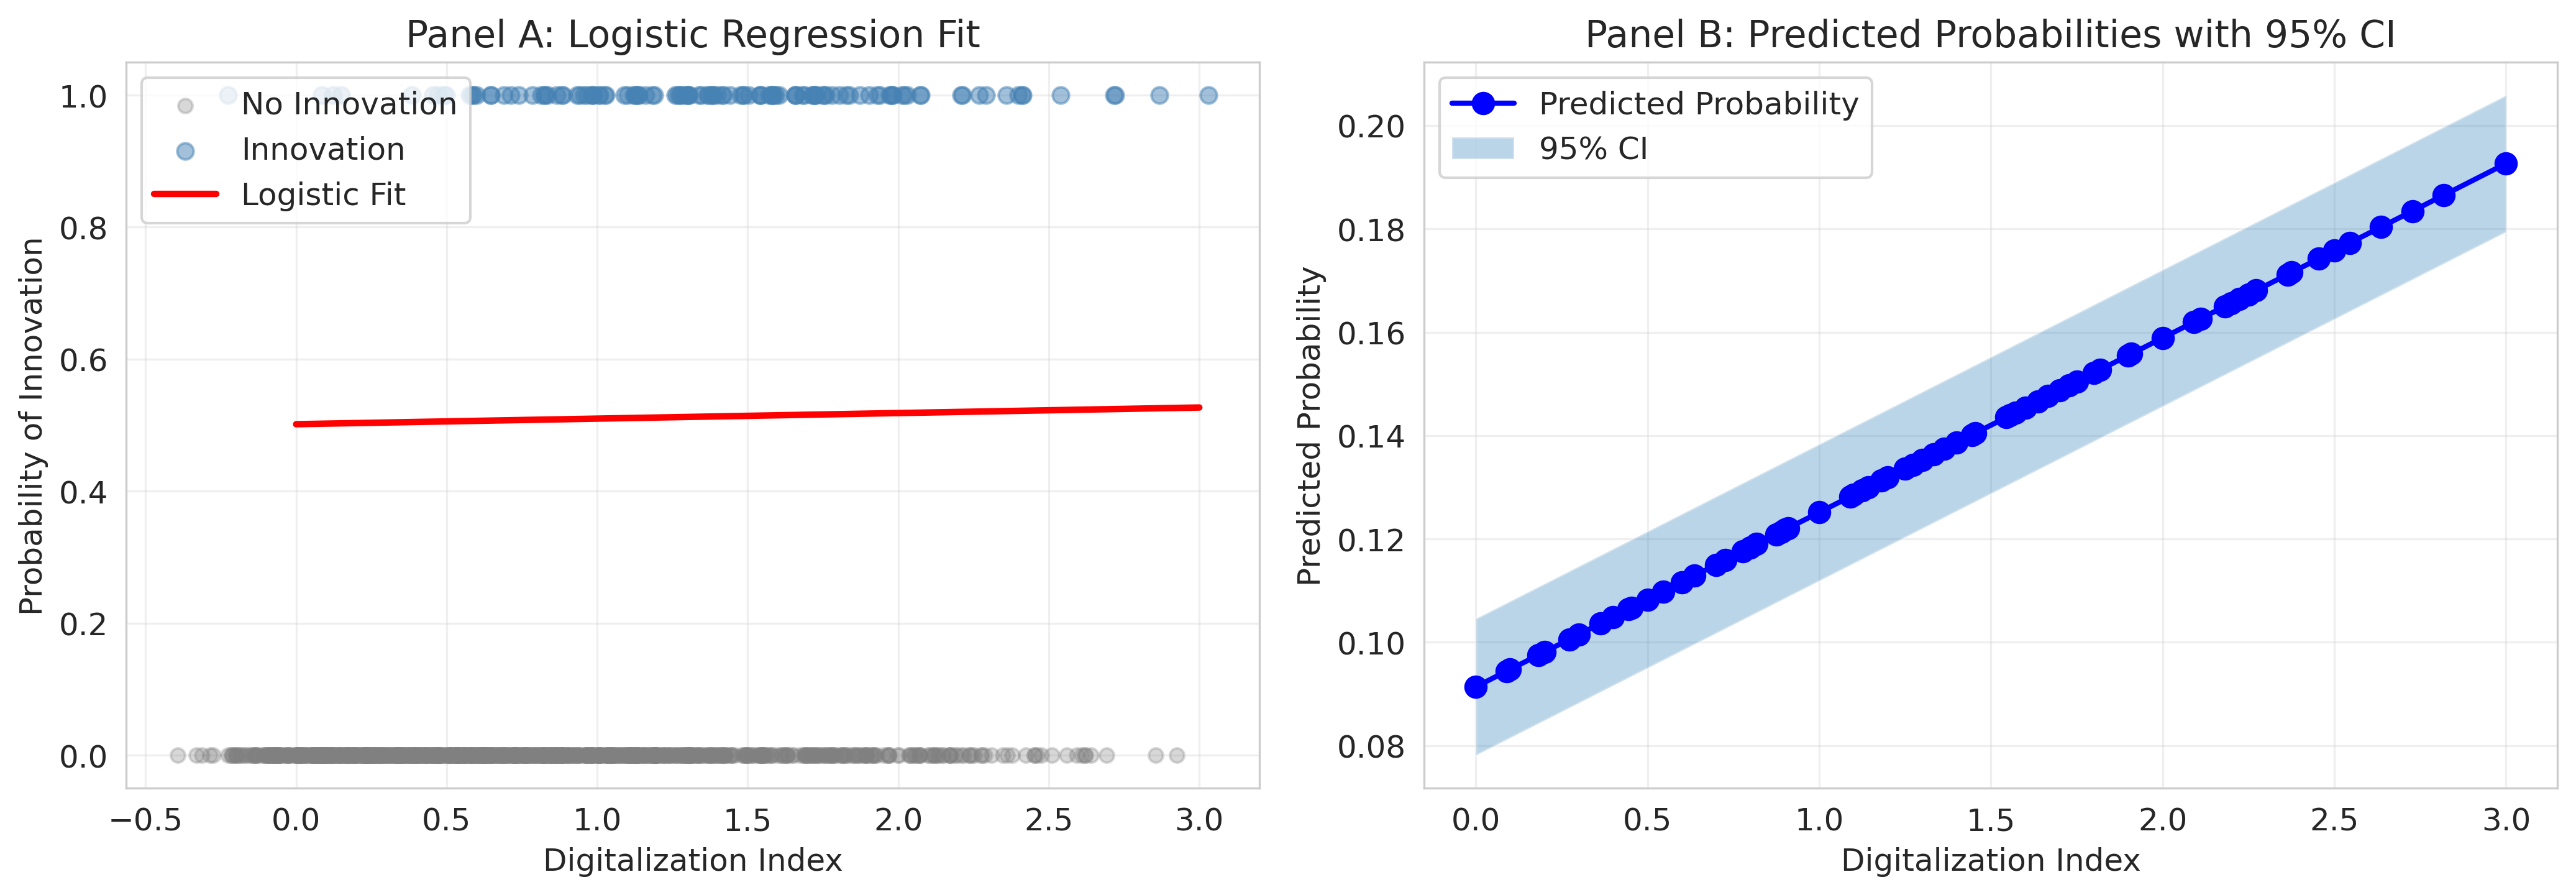
\includegraphics[width=0.9\textwidth]{logistic_regression_plot}
\caption{Logistic Regression: Digitalization vs Novel Product Innovation Probability}
\end{figure}

Figure shows:
\begin{itemize}
    \item \textbf{Panel A:} Raw data (jittered) with fitted logistic regression curve. Gray dots = firms without innovation, blue dots = firms with innovation.
    \item \textbf{Panel B:} Predicted probabilities with 95\% confidence intervals across digitalization levels. The line shows a slight upward slope, confirming the positive (but small) effect of digitalization on innovation probability.
\end{itemize}

\section*{Conclusion}

\textbf{Hypothesis SUPPORTED:} Digitalization DOES increase novel product innovation probability (coef = 0.034, p = 0.007).

\textbf{Key findings:}
\begin{itemize}
    \item \textbf{Digitalization matters} -- Firms with higher digital technology adoption are more likely to introduce novel innovations. A one-unit increase in the digitalization index is associated with a 3.4 percentage point increase in innovation probability.
    
    \item \textbf{Quality improvement by process innovations} -- Strong positive effect (coef = 0.557, p $<$ 0.01). Firms that achieve quality improvements through process innovations are significantly more likely to introduce novel products.
    
    \item \textbf{East Germany location} -- Positive effect (coef = 0.052, p $<$ 0.01). East German firms show higher innovation probability.
    
    \item \textbf{Firm size} -- Small positive effect (p $<$ 0.01). Larger firms are slightly more innovative.
    
    \item \textbf{No moderation by firm size} -- The effect of digitalization does not vary significantly with firm size.
\end{itemize}

\textbf{Implications:} Digital technology adoption appears to be an important driver of novel product innovation. Firms investing in digital interconnection, communication tools, e-commerce, and data analytics are better positioned to develop breakthrough innovations.

\vspace{1cm}
\hrule
\vspace{0.5cm}
\small
All analysis conducted in Python using \texttt{pyfixest} (regression), \texttt{marginaleffects} (predictions and plots), and \texttt{ydata-profiling} (data profiling) packages.

\end{document}
